Per quanto riguarda in particolare il sistema di generazione degli overload tramite CFA, esso modella gli overload auto-generati 
grazie alla classe \texttt{CommonFeatureAdoptionPlanDescriptor}. Essa è implementata tramite un variant, un'approccio tipico in C++
il quale non è facilmente rappresentabile in UML. Per rappresentare tale classe quindi, si è scelto di diagrammare una gerarchia 
di classi funzionalmente analoga a quanto implementato. Si tenga a mente dunque che il seguente diagramma è solo a scopo illustrativo,
ma non riflette fedelmente la struttura interna.

\begin{figure}[h]
\vspace{0.5cm}
\begin{adjustwidth}{-2cm}{-2cm} % Adjust left and right margins
\begin{center}
\begin{tikzpicture}[shift={(current page.west)}]
\begin{umlpackage}{model/typesystem}

\umlclass[x=4,y=0, scale=0.6]{CommonFeatureAdoptionPlanDescriptor}{
    ...
}{
    +store\_file\_representation(FileRepresentation) : void \\
    +get\_package\_name\_by\_file\_name(String) : String \\
    +get\_files\_by\_package\_name(String) : List<FileRepresentation> \\
    +get\_imports\_by\_file\_name(String) : List<String>
}

\umlclass[x=0,y=-4,scale=0.6]{RecursiveAdoptionPlan}{
    -argument\_index : Int \\
    -alternatives : List<TypeSignature> \\
    -nested\_plans : List<CommonFeatureAdoptionPlanDescriptor>
}{
    ... 
}

\umlclass[x=9,y=-4,scale=0.6]{DirectAdoptionPlan}{
   -function\_defintion : FunctionDefinition
}{
    ...
}

\umlinherit[geometry=|-]
{DirectAdoptionPlan}
{CommonFeatureAdoptionPlanDescriptor}


\umlinherit[geometry=|-]
{RecursiveAdoptionPlan}
{CommonFeatureAdoptionPlanDescriptor}


\umlaggreg[geometry=-|]
{RecursiveAdoptionPlan}
{CommonFeatureAdoptionPlanDescriptor}

\end{umlpackage}
\end{tikzpicture}
\end{center}
\end{adjustwidth}
\caption{UML-Class-Diagram CommonFeatureAdoptionPlanDescriptor}
\end{figure}
\vspace{0.5cm}

In sede di chiamata di funzione, se il sistema non trova un overload specifico, esso genera un albero che rappresenta tutte le 
possibili combinazioni di tipi attuali per gli argomenti passati in chiamata il cui tipo è una union (anonima e non). \\

Tale albero è costruito tramite nodi di tipo \texttt{CommonFeatureAdoptionPlanDescriptor}, i quali, qualora foglie, rappresentano
una definizione di funzione corrispondente a quella chiamata. Se invece un nodo è di tipo \texttt{RecursiveAdoptionPlan}, esso rappresenta
un dispatch basato sul tipo dell'argomento corrente, e contiene l'indice di tale argomento.

\newpage

Si considerino ad esempio le seguenti definizioni di funzioni:

\vspace{0.5cm}
\begin{lstlisting}[frame=single]
func add(x : Int, y : Int) -> Int {
    return x + y;
}

func add(x : Float, y : Int) -> Float {
    return x + cast<Float>(y);
}

func add(x : Int, y : Float) -> Float {
    return cast<Float>(x) + y;
}

func add(x : Float, y : Float) -> Float {
    return x + y;
}

\end{lstlisting}
\vspace{0.5cm}

Se si effettuasse una chiamata alla funzione \texttt{add}, con due argomenti di tipo \texttt{Int|Float}, il sistema non troverebbe un overload
specifico. Esso genererebbe quindi un albero CFA che rappresenta l'overload generato schematizzabile come segue:

\begin{figure}[h]
    \centering
    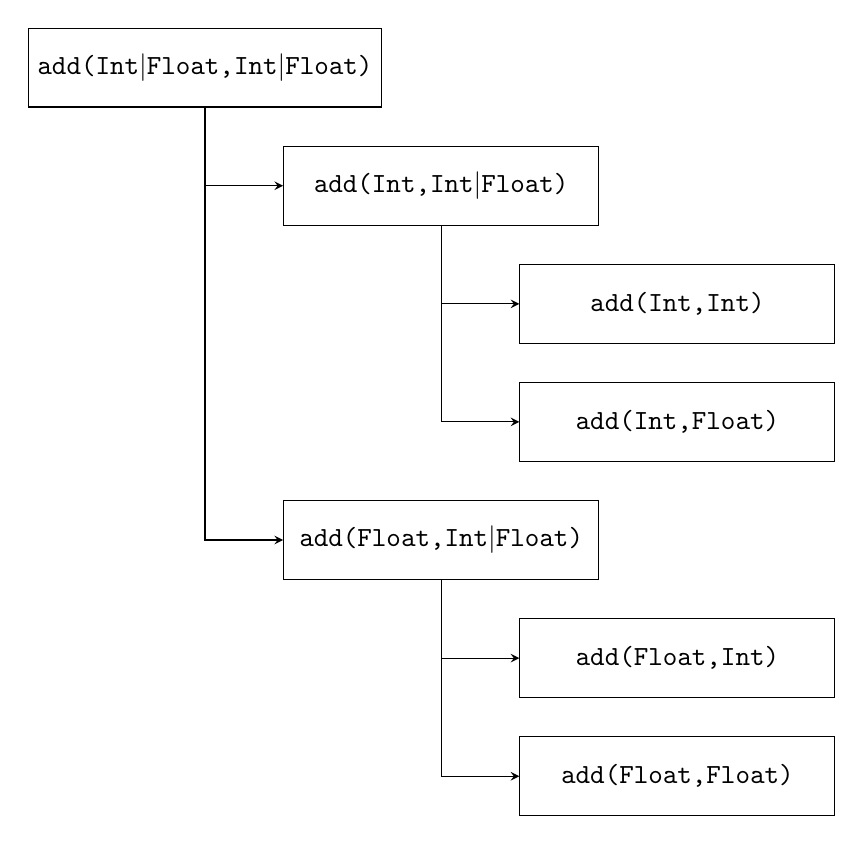
\begin{tikzpicture}[
        box/.style={
            rectangle,
            draw,
            minimum width=4cm,
            minimum height=1cm
        },
        >=stealth
    ]
    
    % Main boxes
    \node[box] (A) at (0,0) {\texttt{add(Int$|$Float,Int$|$Float)}};
    \node[box] (B) at (3,-1.5) {\texttt{add(Int,Int$|$Float)}};
    \node[box] (B1) at (6,-3) {\texttt{add(Int,Int)}};
    \node[box] (B2) at (6,-4.5) {\texttt{add(Int,Float)}};
    \node[box] (C) at (3,-6) {\texttt{add(Float,Int$|$Float)}};
    \node[box] (C1) at (6,-7.5) {\texttt{add(Float,Int)}};
    \node[box] (C2) at (6,-9) {\texttt{add(Float,Float)}};
    
    % Connections
    \draw[->] (A.south) |- (B.west);
    \draw[->] (A.south) |- (C.west);

    \draw[->] (B.south) |- (B1.west);
    \draw[->] (B.south) |- (B2.west);

    \draw[->] (C.south) |- (C1.west);
    \draw[->] (C.south) |- (C2.west);
    
    \end{tikzpicture}
    \caption{Albero CFA per la funzione \texttt{add}}
    \label{fig:overload_tree}
\end{figure}